\documentclass[13pt, usenames, dvipsnames]{beamer}
\usepackage{pgfpages}

%\setbeameroption{show notes on second screen}
\usetheme[progressbar=frametitle,block=fill]{metropolis}

%\usepackage[
%backend=biber,
%style=ieee,
%citestyle=authoryear,
%mincitenames=1,
%maxcitenames=1
%]{biblatex}

\usepackage{alltt}
\usepackage{tikz, verbatimbox}
\usetikzlibrary{arrows, arrows.meta, positioning, decorations.markings, shapes, decorations, overlay-beamer-styles}
\usepackage{xcolor}
\usepackage[utf8]{inputenc}
\usepackage{multicol}
\usepackage{tabularx}
\usepackage{marvosym} 
\usepackage{comment}
\usepackage[ngerman]{babel}

%\addbibresource{bib.bib}

\tikzset{>=Latex}
\tikzset{
  %auto,
  invisible/.style={opacity=0},
  visible on/.style={alt={#1{}{invisible}}},
  alt/.code args={<#1>#2#3}{%
    \alt<#1>{\pgfkeysalso{#2}}{\pgfkeysalso{#3}} % \pgfkeysalso doesn't change the path
  },
}

\newcommand\Wider[2][2.0cm]{%
\makebox[\linewidth][c]{%
  \begin{minipage}{\dimexpr\textwidth+#1\relax}
  \raggedright#2
  \end{minipage}%
  }%
}

\title{ôbstsalat}
\subtitle{Explorative Stadterkundung mit offenen Daten}
\author{Roland, Jurkschat, Do Duc, de Boer}

\begin{document}

\frame{\titlepage}

\begin{frame}{Offene Daten für personalisierte Stadexploration}
    \begin{minipage}{.5\textwidth}
        \only<1>{\includegraphics[width=\textwidth]{frauenkircheAusblick.png}}
        \only<2>{\includegraphics[width=\textwidth]{großerGarten.png}}
        \only<3>{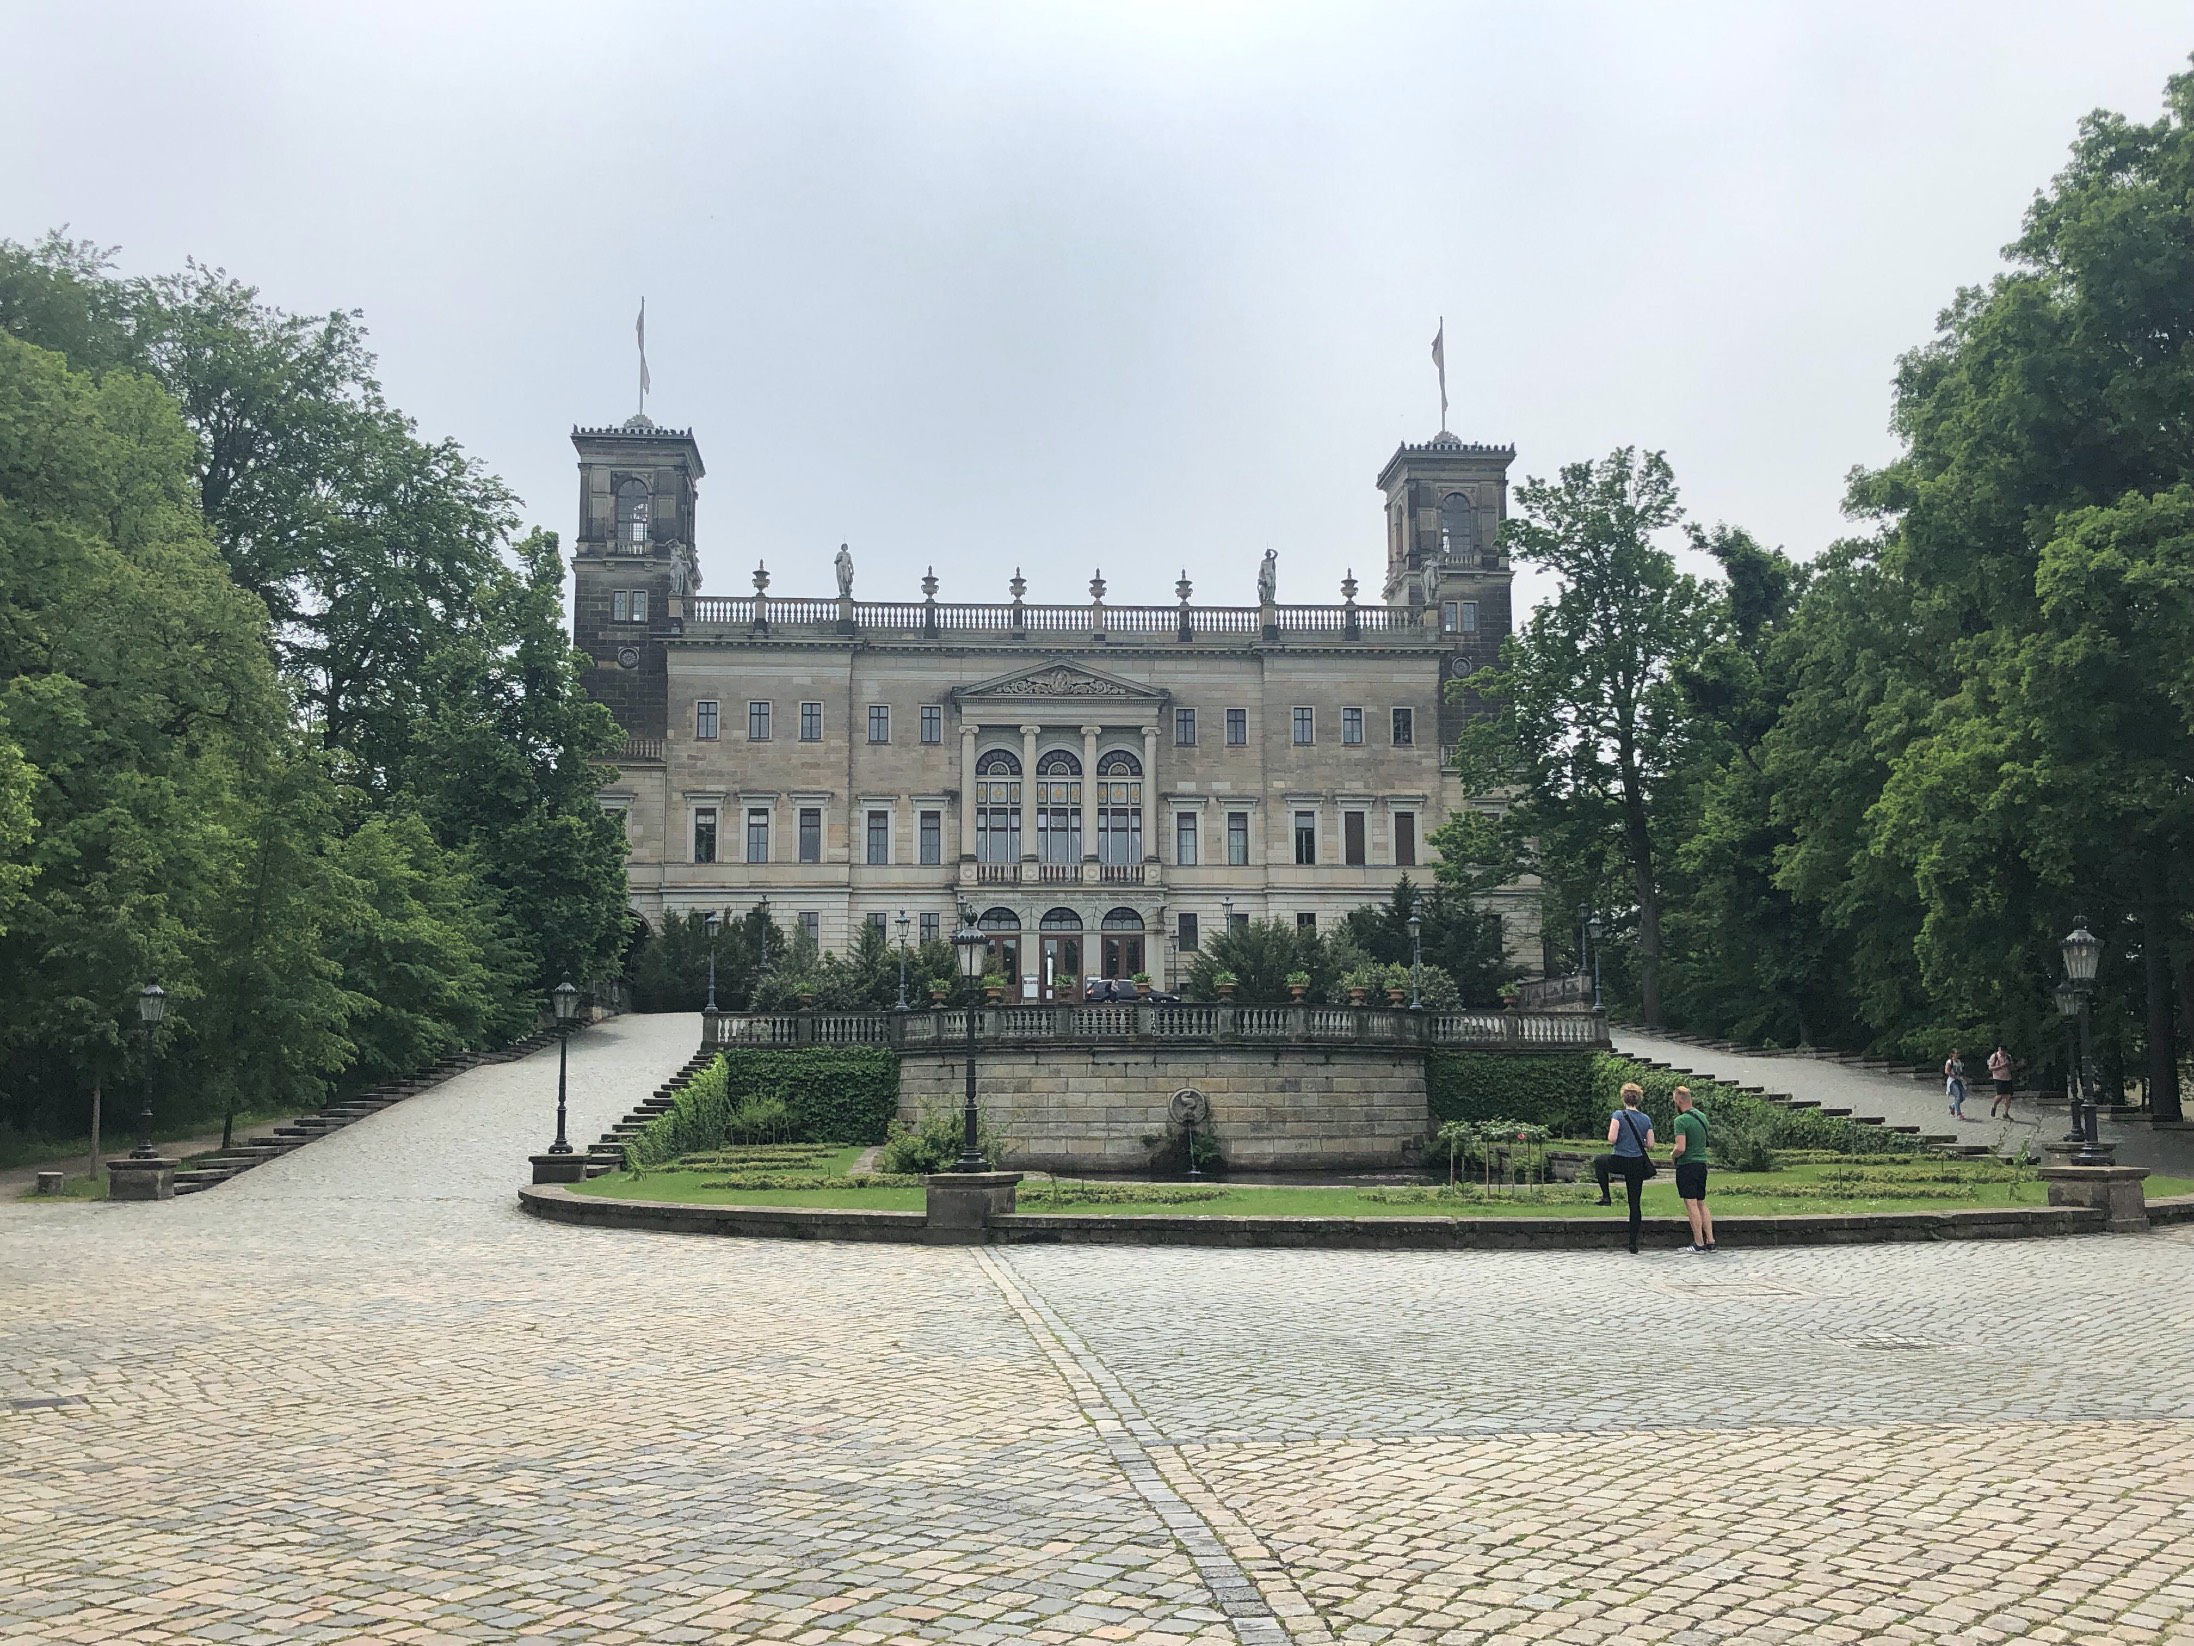
\includegraphics[width=\textwidth]{albrechtsbergSchloss.png}}
    \end{minipage}%
    \begin{minipage}{.5\textwidth}
        \begin{itemize}
            \item Erkunde deine Stadt auf neuen Wegen
                \pause
            \item Genieße deinen Aufenthalt und sieh Dresden im Detail
                \pause
            \item Mache interessante Orte sichtbar
        \end{itemize}
    \end{minipage}
\end{frame}

\begin{frame}{Rundrouten}
	ôbstsalat plant Rundrouten die:
	\begin{itemize}
		\item von einem selbstgewähltem Standort aus starten
		\item Stationen präferierter Themenbereiche verbinden
		\item das individuelle Zeitbudget berücksichtigen
	\end{itemize}
\end{frame}

\begin{frame}{Wen wollen wir erreichen?}
    \begin{itemize}
        \item Einheimische, die Dresden neu entdecken wollen.
        \item Touristen, die für sie interessante Ziele besuchen wollen.
        \item Die Stadt als Anbieter / Planer für kulturelle Stadttouren.
    \end{itemize}
\end{frame}

\begin{frame}{}
    \Wider{
    \centering
    \begin{tikzpicture}
        \node (data) at (-4.5, 0) {\includegraphics[width=.2\textwidth]{openData.png}};
        \node (datal) at (-4.5, -1.5) {Datenauswahl};
        \node (preproc) at (0, .5) {\includegraphics[width=.2\textwidth]{openrouteservice.png}};
        \node (routing) at (0, -.5) {\includegraphics[width=.2\textwidth]{googleai.png} };
        \node (routingl) at (0, -1.5) {Vorverarbeitung \& Routing};
        \node (vis) at (4.5, 0) {\includegraphics[width=.2\textwidth]{leaflet.png}};
        \node (visl) at (4.5, -1.5) {Visualisierung};

        \draw[->] (data) -- (-1.5, 0);
        \draw[->] (1.5, 0) -- (vis);
    \end{tikzpicture}
}
\end{frame}
\end{document}
